\documentclass{standalone}
\usepackage{tikz}
\usetikzlibrary{patterns, positioning}


\begin{document}
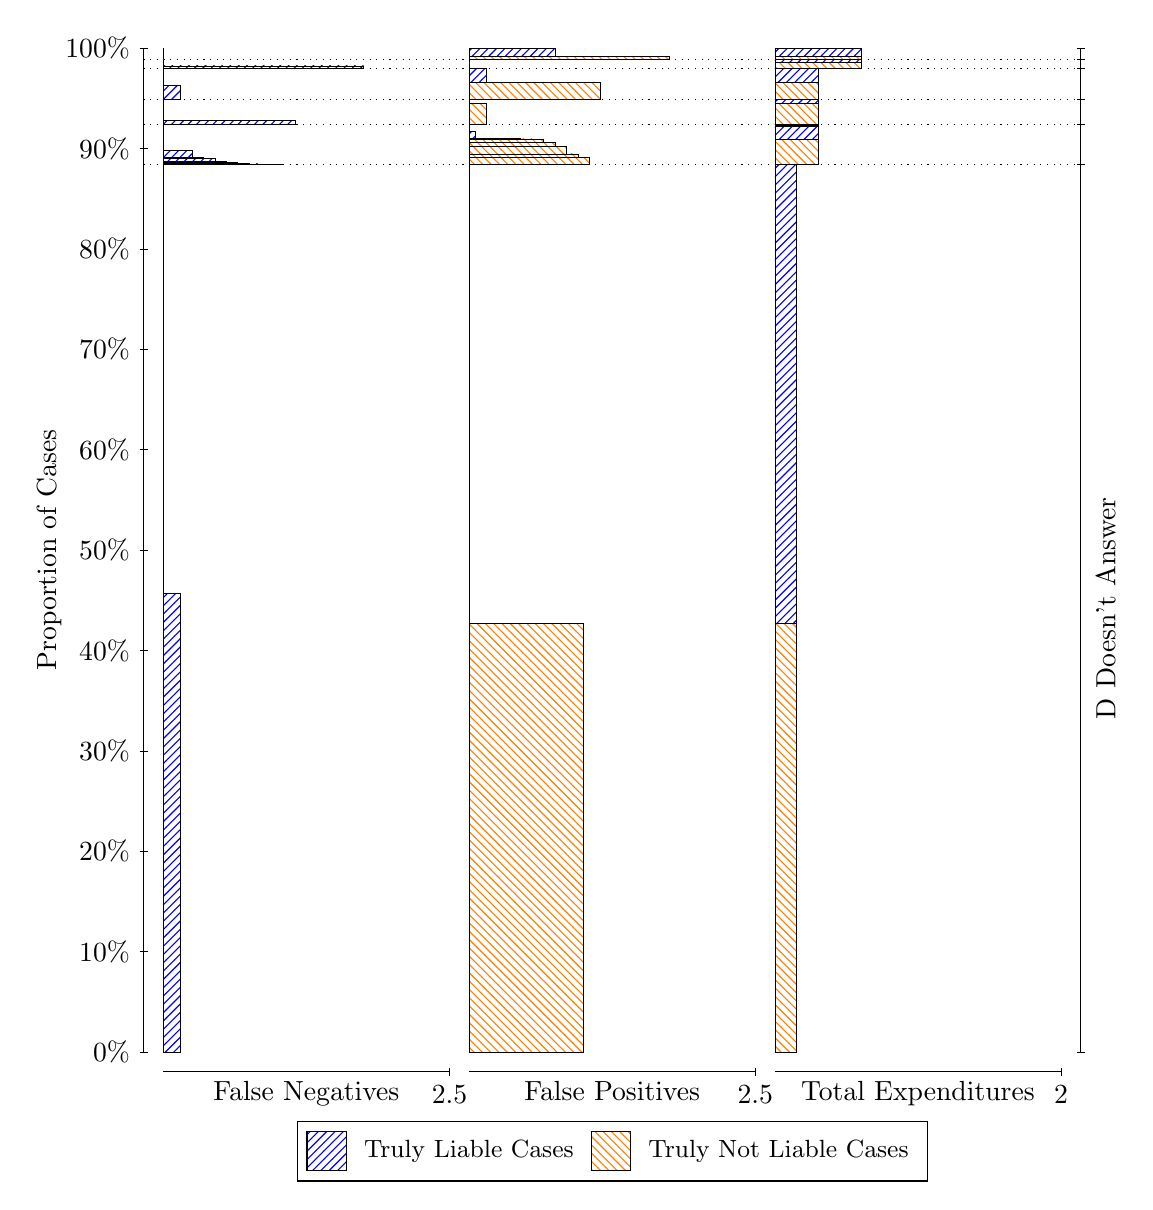
\begin{tikzpicture}
\draw[black, very thin] (1.5,1.75) -- (1.5,14.5);
\node[rotate=90, text=black, anchor=center] at (0.3, 8.125) {Proportion of Cases};
\draw[black, very thin] (1.45,1.75) -- (1.55,1.75);
\node[text=black, anchor=east] at (1.45, 1.75) {0\%};
\draw[black, very thin] (1.45,3.025) -- (1.55,3.025);
\node[text=black, anchor=east] at (1.45, 3.025) {10\%};
\draw[black, very thin] (1.45,4.3) -- (1.55,4.3);
\node[text=black, anchor=east] at (1.45, 4.3) {20\%};
\draw[black, very thin] (1.45,5.575) -- (1.55,5.575);
\node[text=black, anchor=east] at (1.45, 5.575) {30\%};
\draw[black, very thin] (1.45,6.85) -- (1.55,6.85);
\node[text=black, anchor=east] at (1.45, 6.85) {40\%};
\draw[black, very thin] (1.45,8.125) -- (1.55,8.125);
\node[text=black, anchor=east] at (1.45, 8.125) {50\%};
\draw[black, very thin] (1.45,9.4) -- (1.55,9.4);
\node[text=black, anchor=east] at (1.45, 9.4) {60\%};
\draw[black, very thin] (1.45,10.675) -- (1.55,10.675);
\node[text=black, anchor=east] at (1.45, 10.675) {70\%};
\draw[black, very thin] (1.45,11.95) -- (1.55,11.95);
\node[text=black, anchor=east] at (1.45, 11.95) {80\%};
\draw[black, very thin] (1.45,13.225) -- (1.55,13.225);
\node[text=black, anchor=east] at (1.45, 13.225) {90\%};
\draw[black, very thin] (1.45,14.5) -- (1.55,14.5);
\node[text=black, anchor=east] at (1.45, 14.5) {100\%};

\draw[black, very thin] (13.4,1.75) -- (13.4,14.5);
\draw[black, very thin] (13.35,1.75) -- (13.45,1.75);
\node[anchor=west] at (13.35, 1.75) {};
\draw[black, very thin] (13.35,13.022) -- (13.45,13.022);
\node[anchor=west] at (13.35, 13.022) {};
\draw[black, very thin] (13.35,13.531) -- (13.45,13.531);
\node[anchor=west] at (13.35, 13.531) {};
\draw[black, very thin] (13.35,13.847) -- (13.45,13.847);
\node[anchor=west] at (13.35, 13.847) {};
\draw[black, very thin] (13.35,14.237) -- (13.45,14.237);
\node[anchor=west] at (13.35, 14.237) {};
\draw[black, very thin] (13.35,14.354) -- (13.45,14.354);
\node[anchor=west] at (13.35, 14.354) {};
\draw[black, very thin] (13.35,14.5) -- (13.45,14.5);
\node[anchor=west] at (13.35, 14.5) {};

\draw[black, very thin, pattern color=blue, pattern=north east lines] (1.75,1.75) rectangle (1.968,7.5776);
\draw[black, very thin, pattern color=orange, pattern=north west lines] (1.75,7.5776) rectangle (1.75,13.022);
\draw[black, very thin, pattern color=blue, pattern=north east lines] (1.75,13.022) rectangle (3.276,13.024);
\draw[black, very thin, pattern color=blue, pattern=north east lines] (1.75,13.024) rectangle (3.1307,13.026);
\draw[black, very thin, pattern color=blue, pattern=north east lines] (1.75,13.026) rectangle (2.9853,13.029);
\draw[black, very thin, pattern color=blue, pattern=north east lines] (1.75,13.029) rectangle (2.84,13.033);
\draw[black, very thin, pattern color=blue, pattern=north east lines] (1.75,13.033) rectangle (2.6947,13.047);
\draw[black, very thin, pattern color=blue, pattern=north east lines] (1.75,13.047) rectangle (2.5493,13.062);
\draw[black, very thin, pattern color=blue, pattern=north east lines] (1.75,13.062) rectangle (2.404,13.094);
\draw[black, very thin, pattern color=blue, pattern=north east lines] (1.75,13.094) rectangle (2.2587,13.113);
\draw[black, very thin, pattern color=blue, pattern=north east lines] (1.75,13.113) rectangle (2.1133,13.196);
\draw[black, very thin, pattern color=orange, pattern=north west lines] (1.75,13.196) rectangle (1.75,13.531);
\draw[black, very thin, pattern color=blue, pattern=north east lines] (1.75,13.531) rectangle (3.4213,13.583);
\draw[black, very thin, pattern color=orange, pattern=north west lines] (1.75,13.583) rectangle (1.75,13.847);
\draw[black, very thin, pattern color=blue, pattern=north east lines] (1.75,13.847) rectangle (1.968,14.023);
\draw[black, very thin, pattern color=orange, pattern=north west lines] (1.75,14.023) rectangle (1.75,14.237);
\draw[black, very thin, pattern color=blue, pattern=north east lines] (1.75,14.237) rectangle (4.2933,14.272);
\draw[black, very thin, pattern color=orange, pattern=north west lines] (1.75,14.272) rectangle (1.75,14.354);
\draw[black, very thin, pattern color=orange, pattern=north west lines] (1.75,14.354) rectangle (1.75,14.389);
\draw[black, very thin, pattern color=blue, pattern=north east lines] (1.75,14.389) rectangle (1.75,14.5);
\draw[black, very thin, pattern color=orange, pattern=north west lines] (5.6333,1.75) rectangle (7.0867,7.1947);
\draw[black, very thin, pattern color=blue, pattern=north east lines] (5.6333,7.1947) rectangle (5.6333,13.022);
\draw[black, very thin, pattern color=orange, pattern=north west lines] (5.6333,13.022) rectangle (7.1593,13.111);
\draw[black, very thin, pattern color=orange, pattern=north west lines] (5.6333,13.111) rectangle (7.014,13.156);
\draw[black, very thin, pattern color=orange, pattern=north west lines] (5.6333,13.156) rectangle (6.8687,13.248);
\draw[black, very thin, pattern color=orange, pattern=north west lines] (5.6333,13.248) rectangle (6.7233,13.297);
\draw[black, very thin, pattern color=orange, pattern=north west lines] (5.6333,13.297) rectangle (6.578,13.34);
\draw[black, very thin, pattern color=orange, pattern=north west lines] (5.6333,13.34) rectangle (6.4327,13.343);
\draw[black, very thin, pattern color=orange, pattern=north west lines] (5.6333,13.343) rectangle (6.4327,13.346);
\draw[black, very thin, pattern color=orange, pattern=north west lines] (5.6333,13.346) rectangle (6.2873,13.352);
\draw[black, very thin, pattern color=orange, pattern=north west lines] (5.6333,13.352) rectangle (6.142,13.354);
\draw[black, very thin, pattern color=orange, pattern=north west lines] (5.6333,13.354) rectangle (5.9967,13.357);
\draw[black, very thin, pattern color=blue, pattern=north east lines] (5.6333,13.357) rectangle (5.706,13.44);
\draw[black, very thin, pattern color=blue, pattern=north east lines] (5.6333,13.44) rectangle (5.6333,13.531);
\draw[black, very thin, pattern color=orange, pattern=north west lines] (5.6333,13.531) rectangle (5.8513,13.795);
\draw[black, very thin, pattern color=blue, pattern=north east lines] (5.6333,13.795) rectangle (5.6333,13.847);
\draw[black, very thin, pattern color=orange, pattern=north west lines] (5.6333,13.847) rectangle (7.3047,14.061);
\draw[black, very thin, pattern color=blue, pattern=north east lines] (5.6333,14.061) rectangle (5.8513,14.237);
\draw[black, very thin, pattern color=orange, pattern=north west lines] (5.6333,14.237) rectangle (5.6333,14.319);
\draw[black, very thin, pattern color=blue, pattern=north east lines] (5.6333,14.319) rectangle (5.6333,14.354);
\draw[black, very thin, pattern color=orange, pattern=north west lines] (5.6333,14.354) rectangle (8.1767,14.389);
\draw[black, very thin, pattern color=blue, pattern=north east lines] (5.6333,14.389) rectangle (6.7233,14.5);
\draw[black, very thin, pattern color=orange, pattern=north west lines] (9.5167,1.75) rectangle (9.7892,7.1947);
\draw[black, very thin, pattern color=blue, pattern=north east lines] (9.5167,7.1947) rectangle (9.7892,13.022);
\draw[black, very thin, pattern color=orange, pattern=north west lines] (9.5167,13.022) rectangle (10.062,13.343);
\draw[black, very thin, pattern color=blue, pattern=north east lines] (9.5167,13.343) rectangle (10.062,13.508);
\draw[black, very thin, pattern color=orange, pattern=north west lines] (9.5167,13.508) rectangle (10.062,13.511);
\draw[black, very thin, pattern color=blue, pattern=north east lines] (9.5167,13.511) rectangle (10.062,13.512);
\draw[black, very thin, pattern color=orange, pattern=north west lines] (9.5167,13.512) rectangle (10.062,13.524);
\draw[black, very thin, pattern color=blue, pattern=north east lines] (9.5167,13.524) rectangle (10.062,13.531);
\draw[black, very thin, pattern color=orange, pattern=north west lines] (9.5167,13.531) rectangle (10.062,13.795);
\draw[black, very thin, pattern color=blue, pattern=north east lines] (9.5167,13.795) rectangle (10.062,13.847);
\draw[black, very thin, pattern color=orange, pattern=north west lines] (9.5167,13.847) rectangle (10.062,14.061);
\draw[black, very thin, pattern color=blue, pattern=north east lines] (9.5167,14.061) rectangle (10.062,14.237);
\draw[black, very thin, pattern color=orange, pattern=north west lines] (9.5167,14.237) rectangle (10.607,14.319);
\draw[black, very thin, pattern color=blue, pattern=north east lines] (9.5167,14.319) rectangle (10.607,14.354);
\draw[black, very thin, pattern color=orange, pattern=north west lines] (9.5167,14.354) rectangle (10.607,14.389);
\draw[black, very thin, pattern color=blue, pattern=north east lines] (9.5167,14.389) rectangle (10.607,14.5);
\draw[black, dotted] (1.5,13.022) -- (13.4,13.022);
\draw[black, dotted] (1.5,13.531) -- (13.4,13.531);
\draw[black, dotted] (1.5,13.847) -- (13.4,13.847);
\draw[black, dotted] (1.5,14.237) -- (13.4,14.237);
\draw[black, dotted] (1.5,14.354) -- (13.4,14.354);
\draw[black, very thin] (1.75,1.5) -- (5.3833,1.5);
\node[text=black, anchor=north] at (3.5667, 1.5) {False Negatives};
\draw[black, very thin] (5.3833,1.45) -- (5.3833,1.55);
\node[text=black, anchor=north] at (5.3833, 1.45) {2.5};

\draw[black, very thin] (5.6333,1.5) -- (9.2667,1.5);
\node[text=black, anchor=north] at (7.45, 1.5) {False Positives};
\draw[black, very thin] (9.2667,1.45) -- (9.2667,1.55);
\node[text=black, anchor=north] at (9.2667, 1.45) {2.5};

\draw[black, very thin] (9.5167,1.5) -- (13.15,1.5);
\node[text=black, anchor=north] at (11.333, 1.5) {Total Expenditures};
\draw[black, very thin] (13.15,1.45) -- (13.15,1.55);
\node[text=black, anchor=north] at (13.15, 1.45) {2};

\node[text=black, centered, rotate=90] at (13.72, 7.3861) {D Doesn't Answer};






\draw (7.449999999999999,1.5) node[draw=none] (baseCoordinate) {};
\begin{scope}[align=center]
        \matrix[scale=0.5, draw=black, below=0.5cm of baseCoordinate, nodes={draw}, column sep=0.1cm]{
            \node[rectangle, draw, minimum width=0.5cm, minimum height=0.5cm, pattern color=blue, pattern=north east lines] {}; &
            \node[draw=none, font=\small, text=black] (B) {Truly Liable Cases}; &
            \node[rectangle, draw, minimum width=0.5cm, minimum height=0.5cm, pattern color=orange, pattern=north west lines] {}; &
            \node[draw=none, font=\small, text=black] (B) {Truly Not Liable Cases}; \\
            };
\end{scope}

\end{tikzpicture}
\end{document}